\documentclass[fleqn, 11pt, a4paper]{article}

\usepackage[utf8]{inputenc}
\usepackage[T1]{fontenc}
\usepackage{lmodern}
\usepackage[a4paper, margin=2cm]{geometry}
\usepackage{graphicx}
\graphicspath{ {images/} }
\usepackage[french]{babel} % used for proper language of automatic text (toc, figure...)
\usepackage{amsmath}
\usepackage{float} % used for positionning of floats at proper positions
\usepackage{tikz}
\usepackage[hidelinks]{hyperref} % used for links and hidelinks for avoiding box around it
\usepackage[page, toc]{appendix}
\usepackage{listings} % used to include code listing
\lstset{literate=
  {á}{{\'a}}1 {é}{{\'e}}1 {í}{{\'i}}1 {ó}{{\'o}}1 {ú}{{\'u}}1
  {Á}{{\'A}}1 {É}{{\'E}}1 {Í}{{\'I}}1 {Ó}{{\'O}}1 {Ú}{{\'U}}1
  {à}{{\`a}}1 {è}{{\`e}}1 {ì}{{\`i}}1 {ò}{{\`o}}1 {ù}{{\`u}}1
  {À}{{\`A}}1 {È}{{\'E}}1 {Ì}{{\`I}}1 {Ò}{{\`O}}1 {Ù}{{\`U}}1
  {ä}{{\"a}}1 {ë}{{\"e}}1 {ï}{{\"i}}1 {ö}{{\"o}}1 {ü}{{\"u}}1
  {Ä}{{\"A}}1 {Ë}{{\"E}}1 {Ï}{{\"I}}1 {Ö}{{\"O}}1 {Ü}{{\"U}}1
  {â}{{\^a}}1 {ê}{{\^e}}1 {î}{{\^i}}1 {ô}{{\^o}}1 {û}{{\^u}}1
  {Â}{{\^A}}1 {Ê}{{\^E}}1 {Î}{{\^I}}1 {Ô}{{\^O}}1 {Û}{{\^U}}1
  {œ}{{\oe}}1 {Œ}{{\OE}}1 {æ}{{\ae}}1 {Æ}{{\AE}}1 {ß}{{\ss}}1
  {ç}{{\c c}}1 {Ç}{{\c C}}1 {ø}{{\o}}1 {å}{{\r a}}1 {Å}{{\r A}}1
  {€}{{\EUR}}1 {£}{{\pounds}}1
}

\setlength\parindent{0pt}  % no indent on new paragraphs
\renewcommand{\arraystretch}{1.5} % used to enlarge tables

\author{Ricardo Araujo\\
  Jean-Louis Tharin\\
  Sydney Pletscher}
\title{MUI\\
Project Voiture\\
 Rapport de conception}
\date{\today}

\begin{document}

\maketitle
\vspace{8cm}
\begin{figure}[H]

\includegraphics[width=8cm]{heig-vd_logo_couleur_format_jpg}
\centering
\end{figure}

\newpage

\tableofcontents

\newpage

\section{Introduction}
	\subsection{Définition}
	Le but est de contrôler un moteur BLDC grâce à un PIC.
	Le moteur peut tourner entre 125 rpm et 15000 rpm.

	
	
\section{Conception du programme principal}
Le programme sera basé sur des interruptions et une machine a états.
Après les initialisations, le programme ne fait rien en dehors des interruptions.
Lors des interruptions, les événements sont envoyés à la machine a états afin de définir le comportement a adopter.

  \subsection{Machine a états}
  \begin{figure}[H]
  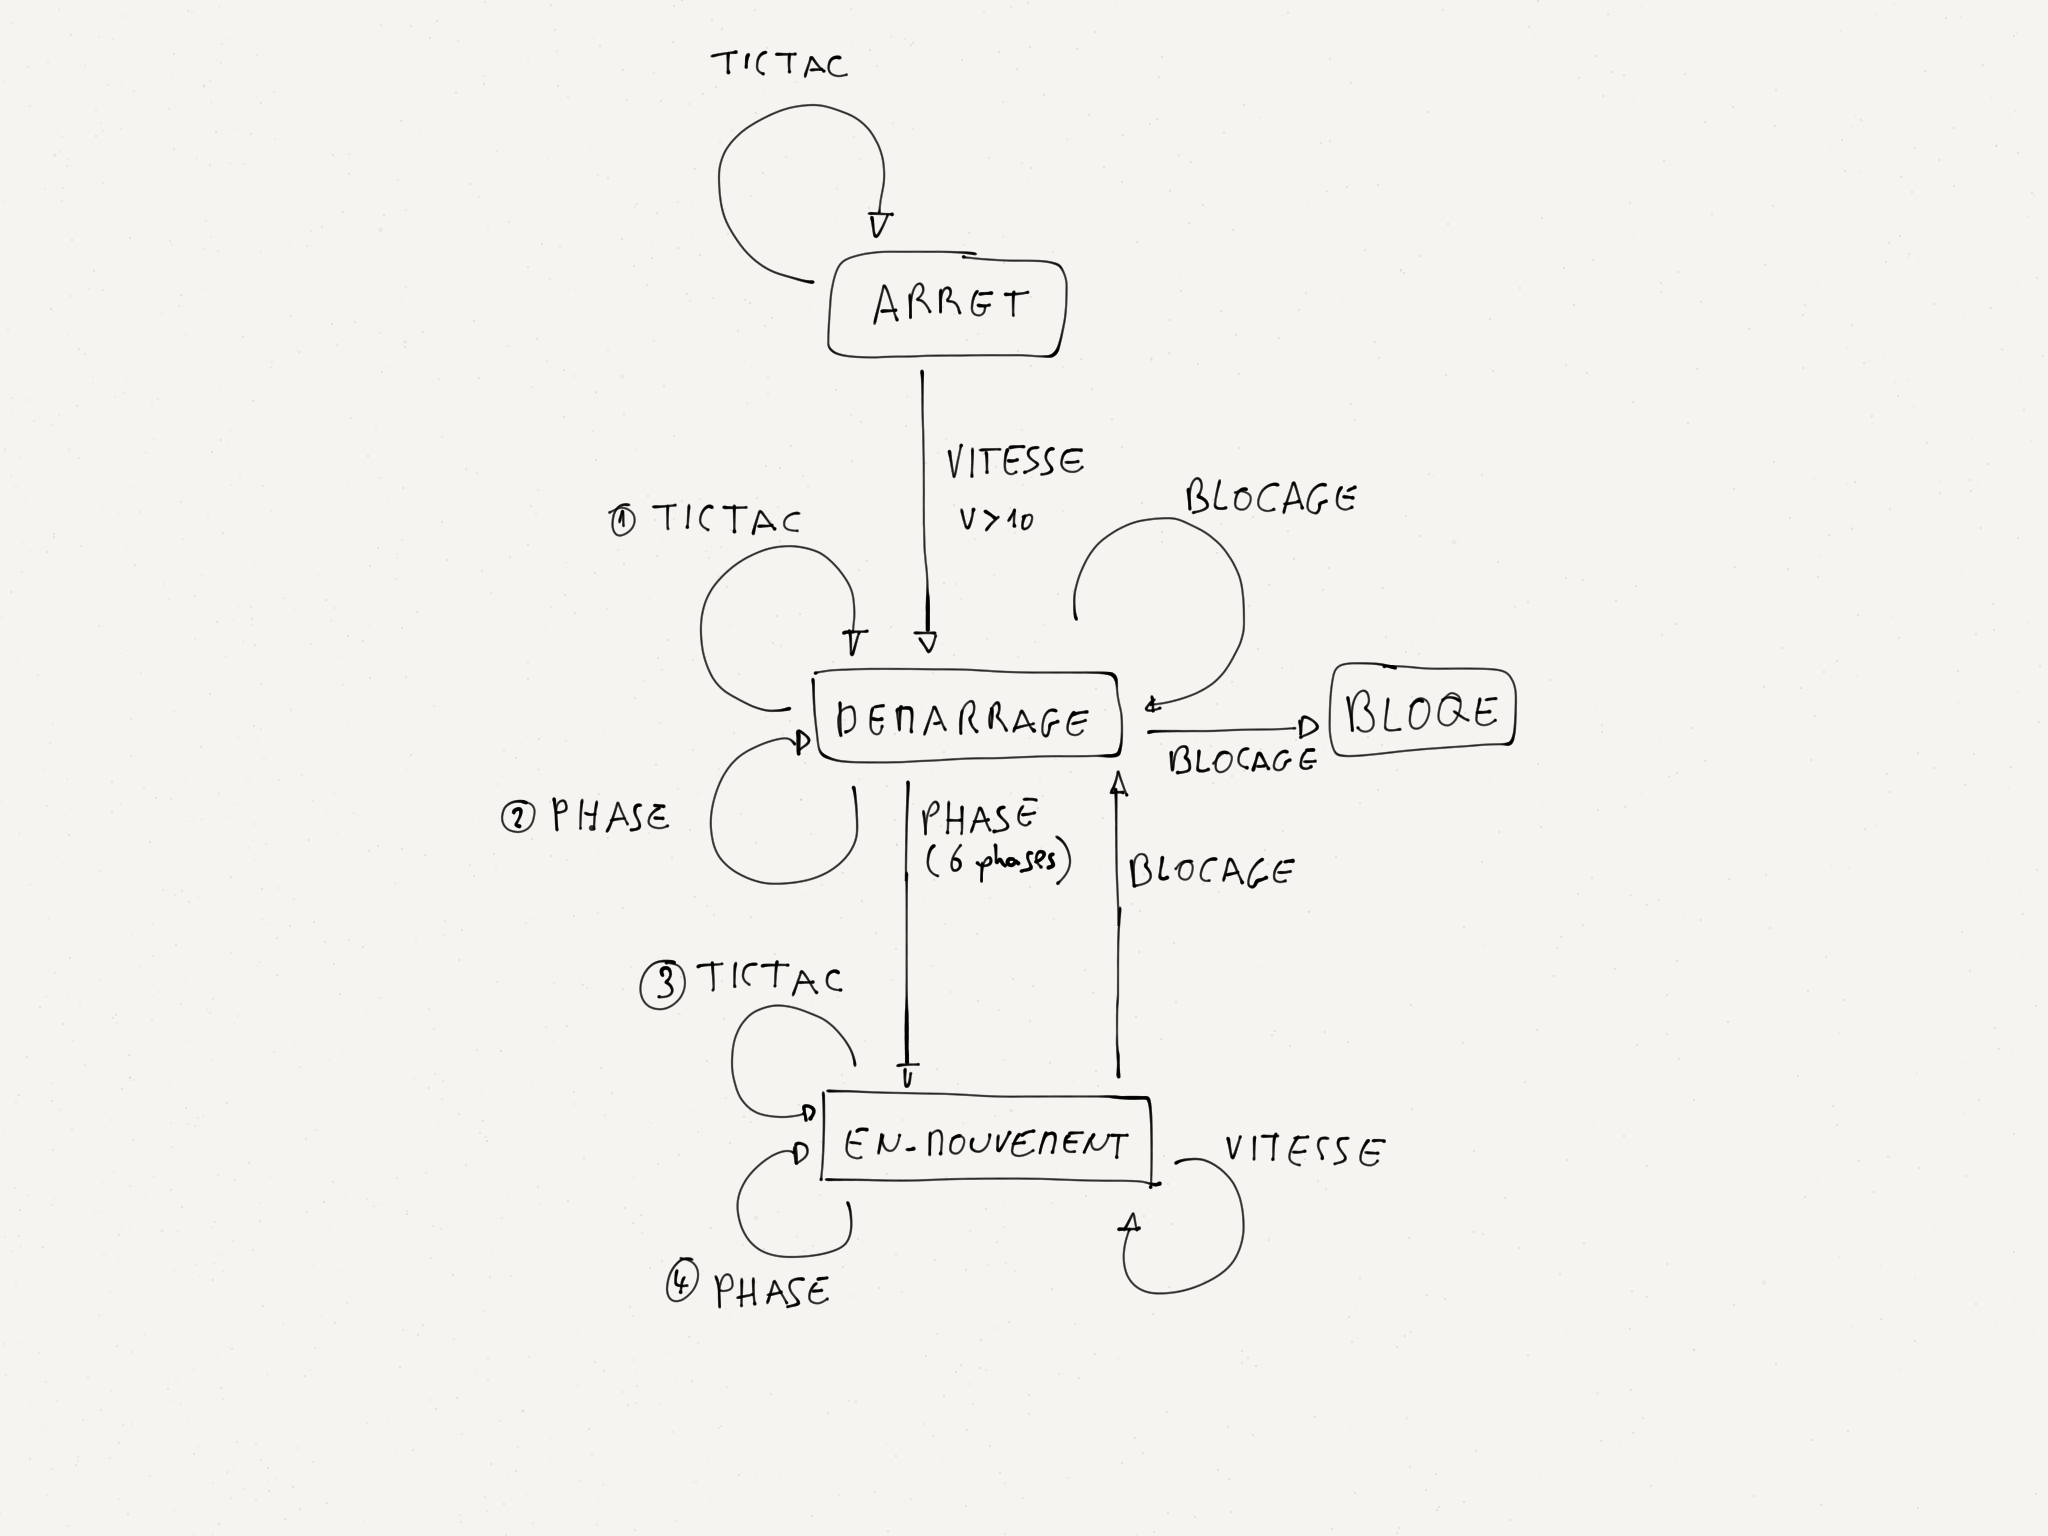
\includegraphics[width=12cm]{state_machine}
  \centering
  \end{figure}

  \subsection{Interfaces}
  \begin{figure}[H]
  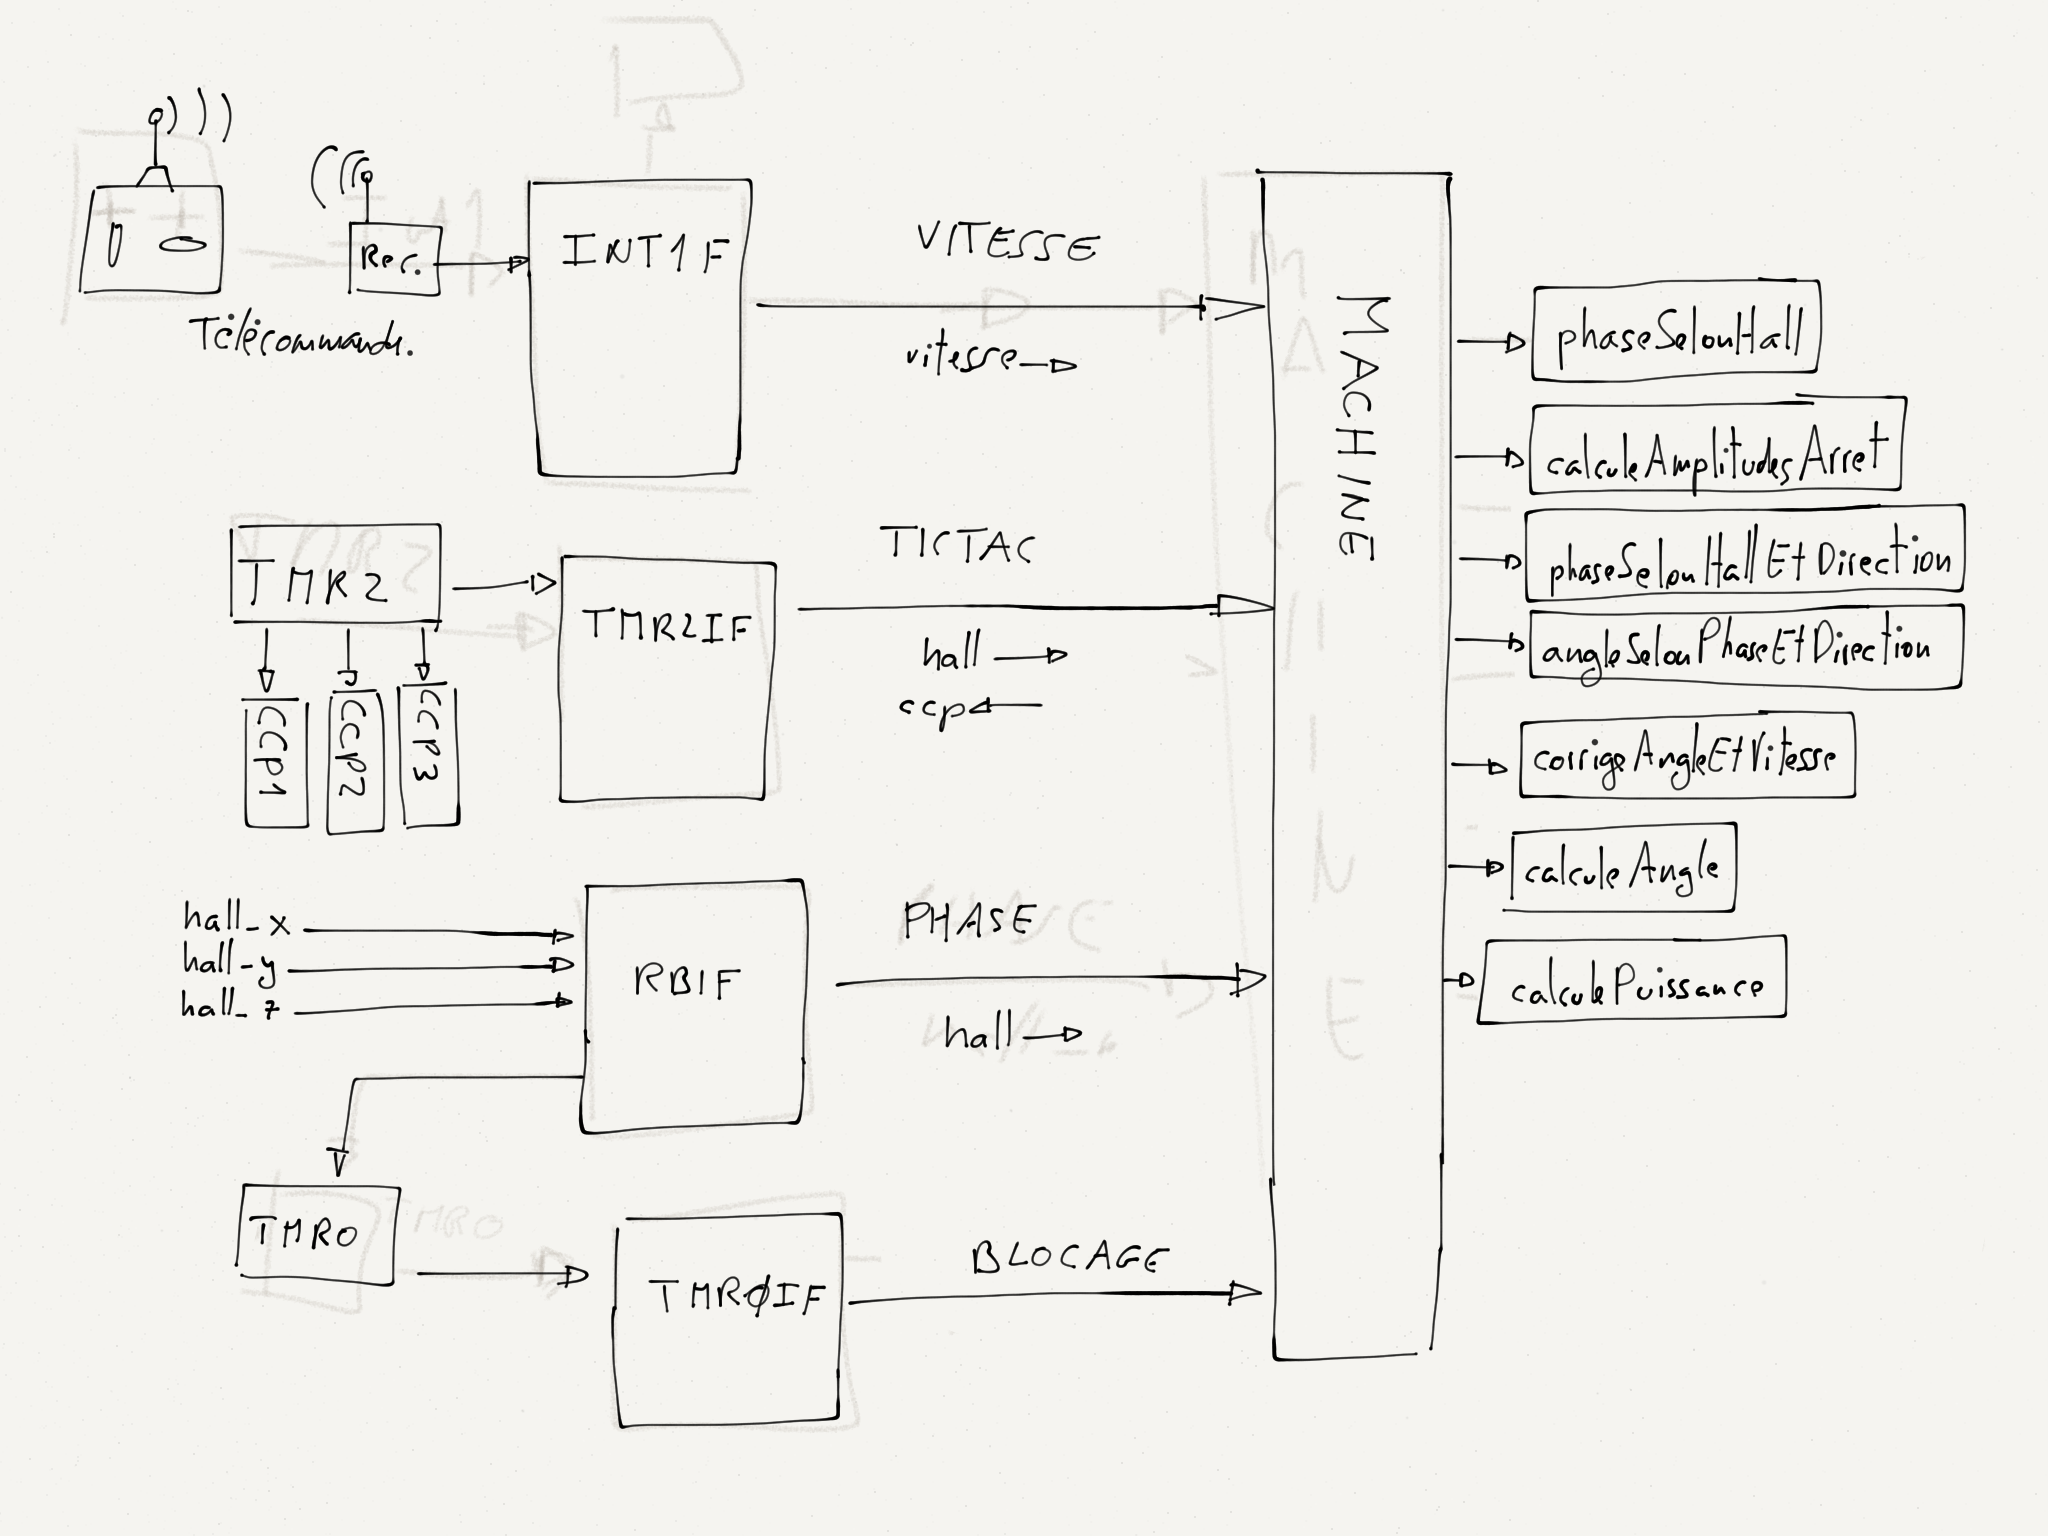
\includegraphics[width=12cm]{main_view_interfaces}
  \centering
  \end{figure}

\section{Calculs d'horloge et des temporisateurs}
  \subsection{Horloge principale}
  L'horloge principale utilisée sera l'horloge interne du PIC à 64MHz.
  Pour cela il faut la configuration suivante:
  \begin{lstlisting}

    #pragma config FOSC = INTIO67  // Oscillateur interne, ports A6 et A7 comme IO.
    #pragma config IESO = OFF      // Pas d'embrouilles avec l'osc. au démarrage.
    #pragma config FCMEN = OFF     // Pas de monitorage de l'oscillateur.

    // configuration de l'horloge
    OSCCONbits.IRCF = 0b111;    // Frequence de base: 16 MHz
    OSCCONbits.SCS = 0b11;      // utilise l'oscillateur interne HFINTOSC
    
    OSCTUNEbits.PLLEN = 1;      // utilise la PLL (horloge x 4)    
  
  \end{lstlisting}
  
  \subsection{Horloge pour les PWM du moteur}
  Nous avons l'horloge principale à 64 MHz et nous voulons 255 niveaux différents possible pour le PWM qui contrôle le moteur.
  Nous devons calculer la fréquence pour le PWM.
  $$F_{PWM} = \frac{F_{OSC}}{4 \cdot TPS \cdot C}$$
  Dans note cas:\\
  $F_{OSC} = 64 MHz$\\
  $C = 256$\\
  et nous voulons la fréquence maximale, donc $TPS = 1$.
  Nous avons donc:
  $$F_{PWM} = \frac{64000000}{4 \cdot 1 \cdot 256} = 62500 = 62.5 [kHz]$$
  Nous avons donc 62500 cycles de PWM par seconde.
  
  \subsection{Cycles selon vitesse}
  Nous avons 6 phases par tour.
  A vitesse maximale de 15000 rpm nous avons:
  $$15000 \ rpm = 250\ tours\ /\ seconde$$
  $$ 250 \ rps = 1500\ phases\ /\ seconde$$
  $$Nb_{cpt} = \frac{cps}{rps} = \frac{62500}{250} = 250\ cycles\ par\ tour$$
  $$Nb_{cpp} = \frac{cps}{pps} = \frac{62500}{1500} = 41.67\ cycles\ par\ phase$$
  A vitesse minimale de 125 rpm nous avons:
  $$125 \ rpm = 2.08\ tours\ /\ seconde$$
  $$ 2.08 \ rps = 12.5\ phases\ /\ seconde$$
  $$Nb_{cpt} = \frac{cps}{rps} = \frac{62500}{2.08} = 30000\ cycles\ par\ tour$$
  $$Nb_{cpp} = \frac{cps}{pps} = \frac{62500}{12.5} = 5000\ cycles\ par\ phase$$
  
  \subsection{Horloge et temporisateur pour la télécommande}
  Une télécommande sera branchée sur INT1 et un signal PWM est reçu.
  Nous utilisons le TMR1 pour la mesure du signal de la télécommande.
  Un signal PWM avec des cycles de 20 ms sera reçu, la vitesse minimale correspond à une pulse de 1 ms, à vitesse 0 une pulse de 1.5 ms et la vitesse maximale est une pulse de 2 ms.
  Nous devons donc utiliser le timer TMR1 pour mesurer des pulse entre 0 et 2ms.

	\newpage
	\begin{appendix}
	\section{Constantes}

	
	\end{appendix}
	
	

\end{document}